\documentclass[12pt,a4paper]{article}
\usepackage[latin1]{inputenc}
\usepackage{amsmath}
\usepackage[T1]{fontenc}
\usepackage{palatino}
\usepackage{amssymb}
\usepackage{graphicx}
\author{Alexandros-Panagiotis Oikonomou}
\setlength{\parindent}{15pt}
\begin{document}
\begin{titlepage}
\begin{center}
\begin{LARGE}
Electronics and Computer Science
Faculty of Physical and Applied Sciences
University of Southampton 
\end{LARGE}
\\[2cm]
\begin{large}
Alexandros-Pana Oikonomou
\\
1$^{st}$ May 2013
\\[2cm]
Solving the Conjugate Gradient Method in a SpiNNaker Machine
\\[3.5cm]
Project Supervisor: Jeff Reeve
\\Second Examiner: Marcus Breede
\\[3.5cm]
A project report submitted for the award of
\\BSc Computer Science
\end{large}
\end{center}
\end{titlepage}
\section*{Abstract}
\pagenumbering{gobble}
SpiNNaker is an asynchronous, event-driven parallel architecture designed to simulate
the human brain. It has been designed to operate as a large scale neural network in
real-time using a System-on-Chip multi core system. Its architecture is different from
usual parallel computers, since cores use spikes to communicate with each other. That
way usual pitfalls of parallel computing, such as race conditions and deadlocks are
avoided. So far the most prominent uses of this architecture have been in
neuroscience and robotics. The aim of this project is to put into use SpiNNaker's
architecture and bring it closer to classic computer science problems, while solving
them optimally. The given algorithm to solve in this project is the conjugate gradient
method, an iterative way of solving systems linear equations. The algorithm successfully runs on the simulator and reduces the time complexity of the most expensive operations of the algorithm.
\newpage
\tableofcontents
\newpage
\section*{Acknowledgments and Statement of Originality}
I would like to thank my supervisor Jeff Reeve for his help and support throughout this project.
\newpage
\section{Introduction}
\pagenumbering{arabic}
\subsection{Aim}
The aim of this project is to correctly solve the Conjugate Gradient Method on a SpiNNaker chip, thus using the massive parallelism that this machine offers to reduce the time complexity of the aforementioned algorithm. This is accomplished by reducing the time complexity of the most expensive operations of the algorithm which are matrix-vector multiplication and the scalar product of vectors. The complexity is reduced dramatically, due to the abundant number of cores provided from the architecture. This report explains this project and its constituents, any background research done to launch this project, along with designe and implementation choices.
\subsection{Reasons and Justification}
\indent
SpiNNaker is an architecture inspired by the biology of the human brain. Its optimal configuration has over a million cores\cite{navaridas2009understanding}, which have mainly been used to simulate the neurons of the human brain and in robotics. Examples of these would be using the SpiNNaker chip to simulate thousands of spiking neurons by using over four million synapses\cite{sharp2012power}, or to simulate the neurons of a retina sensor\cite{davies2010interfacing}.

However little work had been done into using the SpiNNaker architecture to solve classic computer science problems. That is why a problem such as the Conjugate Gradient Method had been proposed, which is a very common solution to optimization problems. In addition to that, the SpiNNaker architecture offers new parallel programming paradigms, that escape some common parallel programming pitfalls such as race conditions, deadlocks, mutual exclusion etc\cite{sharp2011event}.
\subsection{Overview}
Say something here
\newpage
\section{Background}
\subsection{The neuron}
To make the explanation of the SpiNNaker architecture easier, the design from which the SpiNNaker chip was inspired will be outlined. This is no other than the human neuron.

The human neuron is an electrically excitable cell that processes and transmits information through electrical and chemical signals. Its basic costitutes are the the soma, the dendrites and the axon. The soma is the body of the neuron. A dendrite receives signals from the soma of the neuron that it belongs to or other neurons. The dendrite extends for hundreds of micrometers and branches multiple times, thus forming a dendritic tree, which connects with other neurons axons. The axon is used to transmit signals to other neurons and it extends from the soma of the neuron to a dendrite. All human neurons have only one axon. Given the above analysis the dendrites could be described as the inputs of a neuron
\\[0.5cm]
\begin{figure}[h!]
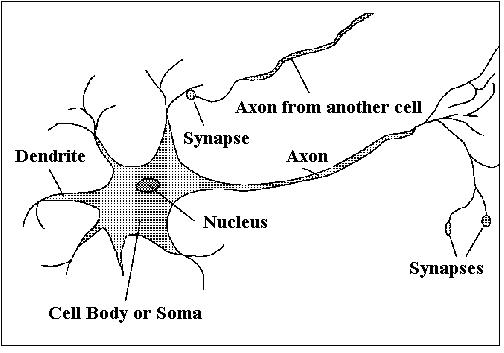
\includegraphics[width=300pt,height=200pt,scale=2]{Pics/neuron.jpg}
\centering
\caption{A neuron}
\end{figure}

One of the most important parts of the neuron structure is the synapse. The synapse is the contact between the axon of a neuron and the dendrite or the soma of another. It is where a information from one neuron is transmitted to the other. When a set of neurons are connected with each other through synapses, then they create a neural network.

Finally, the communication between neurons is accomplihed through spikes, which are either chemichal or electrical\cite{gerstner2002spiking}.

Given the terms in this section, the name of the SpiNNaker chip is detuctable. It stands for Spi(king)N(eural)N(etwork) architecture.
\subsection{The SpiNNaker architecture}
\subsection{The Conjugate Gradient Method}
The conjugate gradient method is an algorithm for the numerical solution of systems of linear eqations of the type Ax=b, those whose matrix is symmetric and positive definite. 

A \emph{symmetric} matrix is a matrix which is equal to its transpose. If A is a symmetric matrix then A=A$^T$. The entries of the matrix are symmetric with respect to the main diagonal, so if an element of the matrix A is a, then a$_{ij}$=a$_{ji}$. 
A \emph{positive definite} matrix M is a matrix which when multipled by any non-zero vector z and its transpose z$^T$, is always positive. In short the relationship that needs to be satisfied is zMz$^T$>0

It is an iterative method, which means it can be applied to sparse systems. A \emph{sparse matrix} is a matrix which is populated primirily with zeros. Its opposite would be a \emph{dense matrix}. It was developed by Magnus Hestenes and Eduard Stiefel and can be used to solve optimization problems\cite{press2007numerical}.
\subsubsection{The quadratic form}
In order to explain why the Conjugate Gradient Method can solve problems whose matrix is positive-definite and symmetric a explanation of the quadratic form needs to be presented.
\begin{center}
\begin{equation}
f(x)=\frac{1}{2}x^TAx-b^T+c
\end{equation}
\end{center}

The gradient f'(x) of the quadratic form would be defined as:

\begin{equation}
f'(x)=\begin{bmatrix}
\frac{df(x)}{dx_1}\cr
\frac{df(x)}{dx_2}\cr
.
.
.\cr
\frac{d(fx)}{d_n}
\end{bmatrix}
\end{equation}

The gradient(2) is a field that for a given point x, indicates the direction where there is a greatest increase of f(x). As it is know from calculus, in order to minimize f(x) the gradient f'(x) must be set to 0.
\newpage
\bibliographystyle{plain}
\bibliography{ref.bib}
\cite{navaridas2009understanding}
\cite{sharp2012power}
\cite{davies2010interfacing}
\cite{sharp2011event}
\cite{gerstner2002spiking}
\cite{press2007numerical}
\end{document}